\begin{figure}
\centering
\begin{subfigure}[b]{0.46\textwidth}
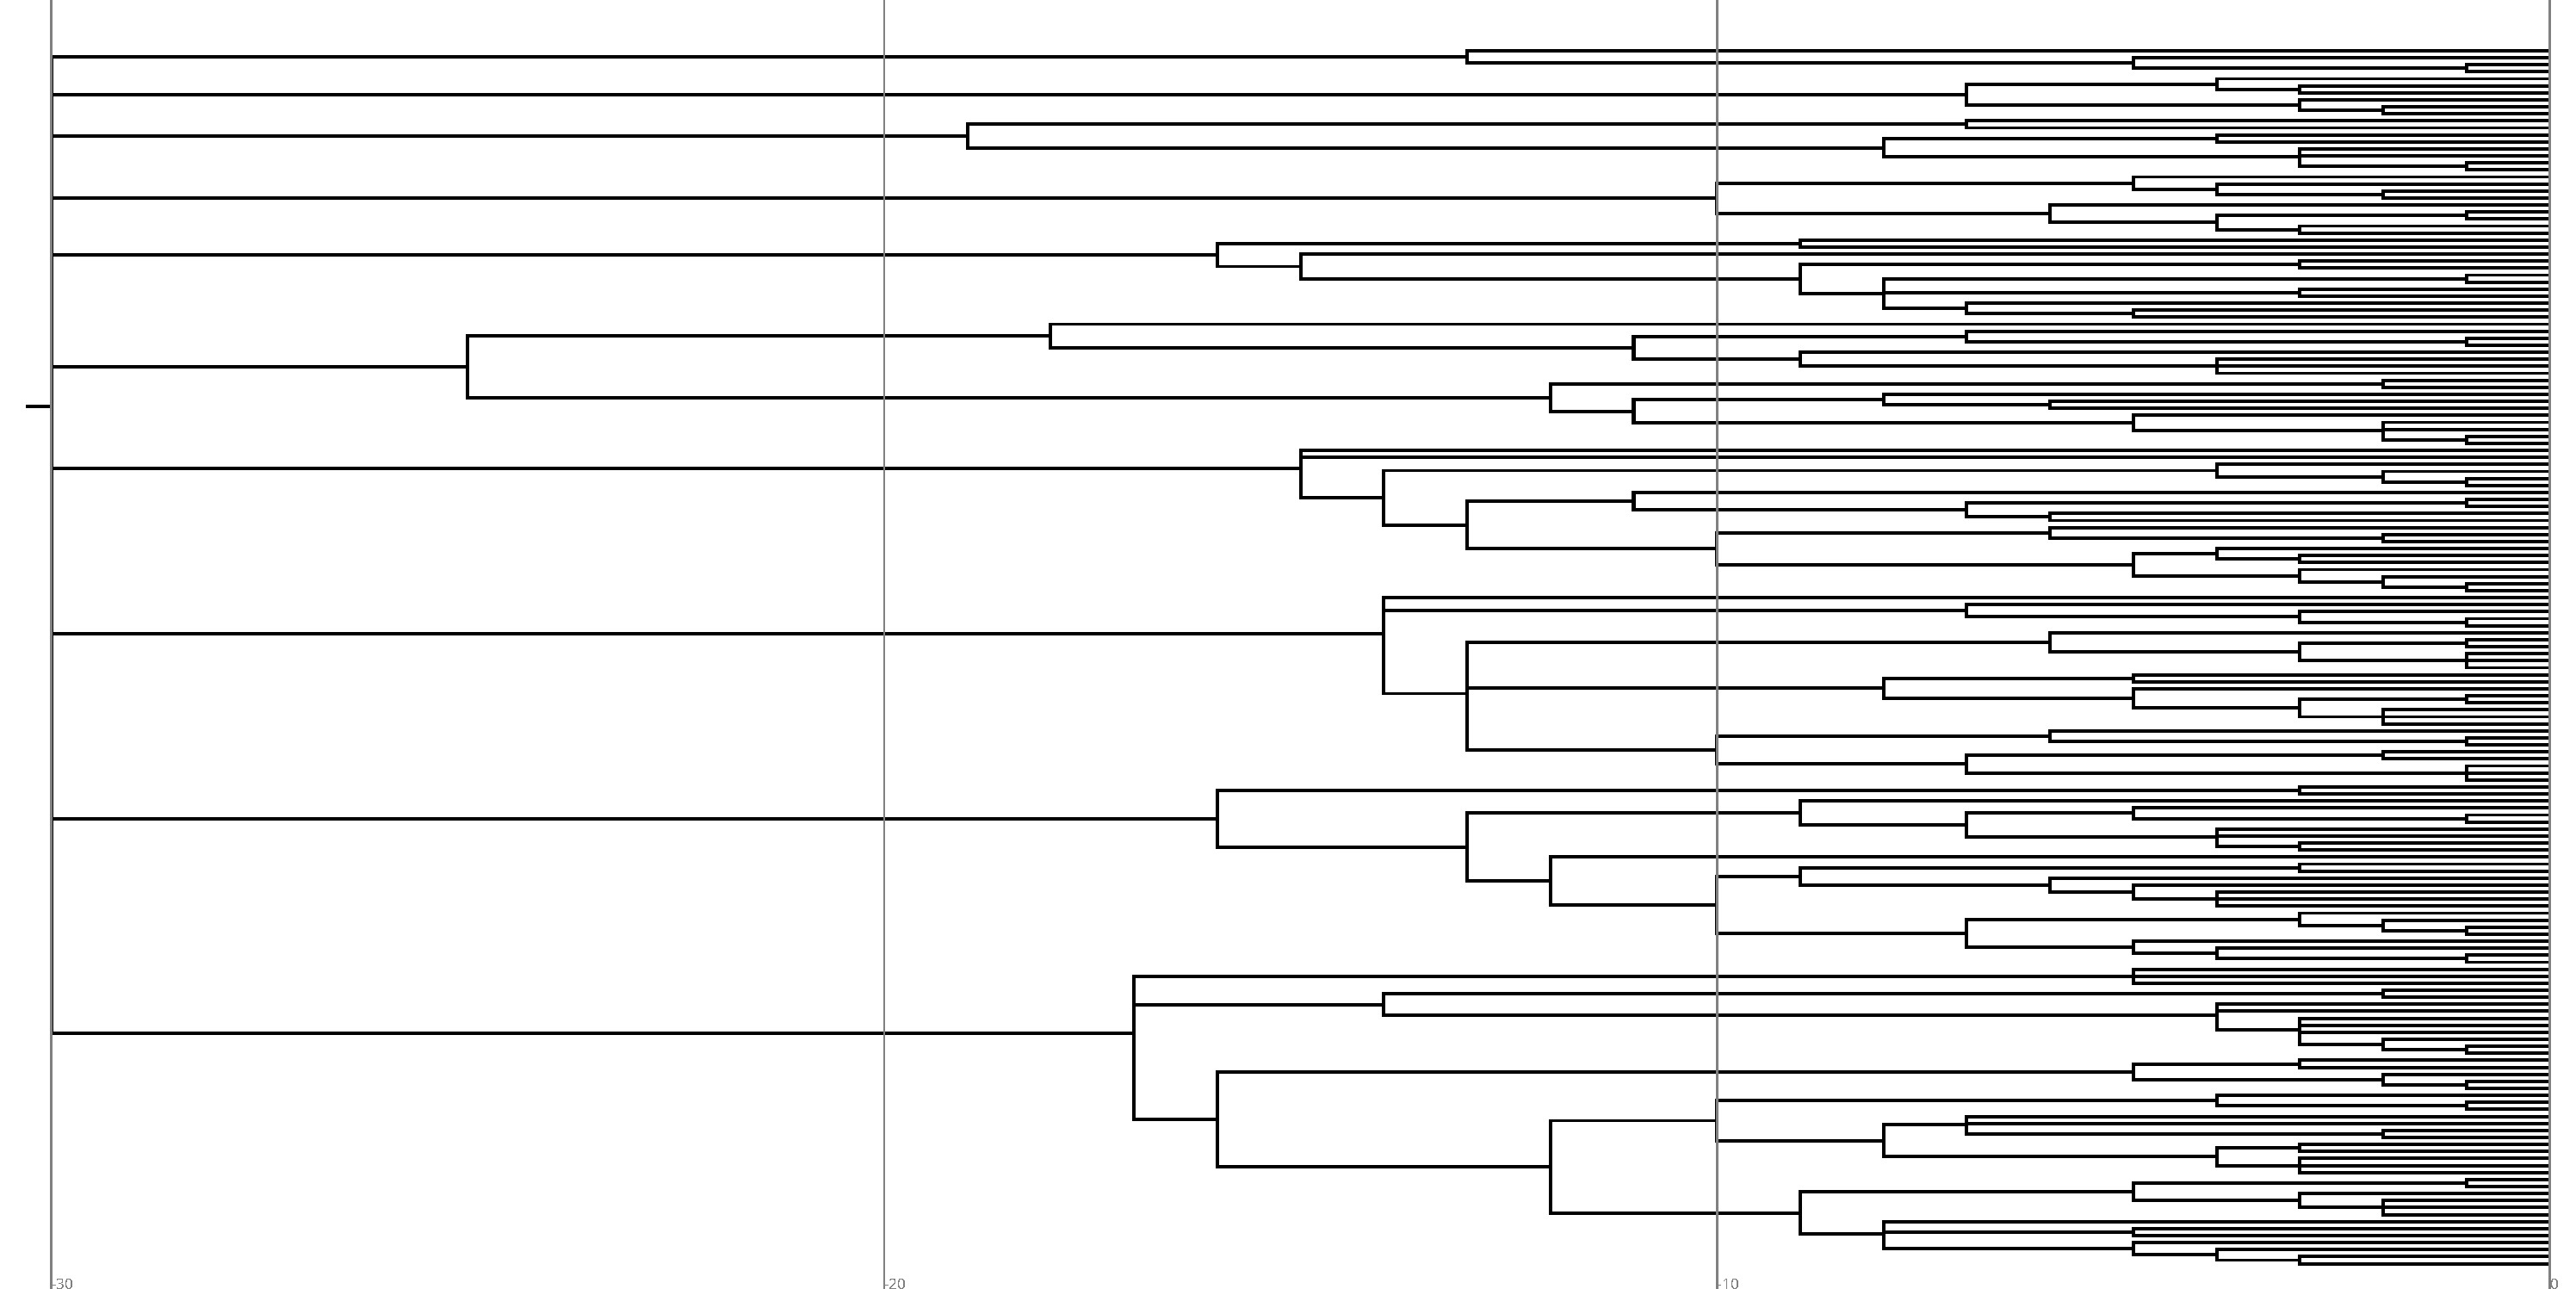
\includegraphics[height=0.12\textheight,width=\textwidth]{img/gen3sis-species/model=gen3sis+taxon=species+treatment=plain+seed=1+phylogeny-snapshot-100000.pdf}
    % \end{noindent}
  \end{subfigure}
  \caption{%
    \textbf{Sample reference phylogeny from Gen3sis under ``plain'' regime.}
    Time axis is linear-scale.
  }
  \label{fig:perfect-tree-phylogeny-gen3sis}
\end{figure}
